% template file include
% A dokumentumosztály megadása a main.tex elején van, hogy az Overleaf feltöltéskor
% a main.tex-et válassza fő fájlnak. Ez a fájl csak a beállításokat tartalmazza.

% szükséges csomagok
\usepackage[utf8]{inputenc}
\usepackage[T1]{fontenc}
\usepackage[magyar]{babel}
\usepackage{float}
\usepackage{graphicx}
\usepackage{pdfpages}
\usepackage{caption}
\usepackage[colorlinks=false, pdfborder={0 0 0}, linkcolor=black, unicode]{hyperref}
\usepackage{mathtools}
\usepackage{relsize}
\usepackage{amsmath}
\usepackage{amsfonts}
\usepackage{amssymb}
\usepackage{listings}
\usepackage{csquotes}
\usepackage{enumitem}
\usepackage{url}
\usepackage[nottoc,numbib]{tocbibind}
\usepackage{titlesec}
\usepackage{titletoc}

% lista elemek közti hely, és vonal mint lista elem előtti jel beállítása
\setlist{nosep, label={--}}

% tartalomjegyzék formázása
\dottedcontents{section}[1.5em]{}{1.5em}{1pc}
\dottedcontents{subsection}[3em]{}{2em}{1pc}
\dottedcontents{subsubsection}[5em]{}{3em}{1pc}

% fejezet cím formázás: 14 pontos betűméret, nagybetűs
% fejezetcím 14 pont, nagybetűs, a lap tetején; a szerző döntése szerint balra igazítva (D18;
% az útmutató 2.3 középre igazítást ír – középre: \filright helyett \filcenter)
\titleformat{\section}{\normalfont\fontsize{14}{17}\selectfont\mdseries\filright\MakeUppercase}{\thesection}{1em}{}
\titleformat{\subsection}{\normalfont\fontsize{12}{12}\bfseries}{\thesubsection}{1em}{}
\titleformat{\subsubsection}{\normalfont\fontsize{12}{12}\bfseries}{\thesubsubsection}{1em}{}

% fejezet cím térközök
\titlespacing*{\section}{0em}{0em}{1em}
\titlespacing*{\subsection}{0em}{1em}{1em}
\titlespacing*{\subsubsection}{0em}{1em}{1em}


% margó (útmutató 2.3): fent 40 mm, lent 25 mm, kívül 25 mm, a kötés oldalán 35 mm;
% az oldalszám fent, középen, a lap szélétől 20 mm-re (a fejléc teteje 20 mm-nél)
\usepackage[right=25mm,
            left=35mm,
            top=40mm,
            bottom=25mm,
            headheight=15pt,
            headsep=14.7mm
            ]{geometry}

% oldalszám a fejlécben, középen
\usepackage{fancyhdr}
% a fejléc 10 mm-rel balra kinyújtva, így az oldalszám a lap (nem a szövegtükör) közepén van
\fancypagestyle{plain}{\fancyhf{}\fancyheadoffset[L]{10mm}\fancyhead[C]{\thepage}\renewcommand{\headrulewidth}{0pt}}
\pagestyle{plain}

% sorköz: 1,5 sor (útmutató 2.3)
\usepackage{setspace}
\onehalfspacing

% times new roman betűtípus
\usepackage{times}

% ábra és táblázat számozás beállítása fejezetenként
\setcounter{figure}{0}
\renewcommand{\thefigure}{\arabic{section}.\arabic{figure}}
\setcounter{table}{0}
\renewcommand{\thetable}{\arabic{section}.\arabic{table}}
\numberwithin{equation}{section}
\numberwithin{figure}{section}

% ábra, táblázat cím formázás
\captionsetup[figure]{labelfont={it, small},textfont={it, small},labelsep=colon}
\captionsetup[table]{labelfont={it, small},textfont={it, small},labelsep=colon}

% hivatkozások formátuma és bib fájl importálása
% útmutató, 1. melléklet: szögletes zárójeles sorszám, az irodalomjegyzék az első szerző szerint
% betűrendben (sorting=nyt), internetes forrásnál az URL és a megtekintés dátuma (url=true, urldate)
\usepackage[backend=biber,style=ieee,sorting=nyt,doi=true,isbn=true,url=true,eprint=false,
            urldate=iso,seconds=true]{biblatex}
\addbibresource{references.bib}
% az útmutató 1. mellékletének szóhasználata: „URL”, „utoljára megtekintve”
\DefineBibliographyStrings{magyar}{url={URL}, urlseen={utoljára megtekintve}}

% bekezdés behúzása
\setlength{\parindent}{5 mm}

% bekezdés térköz
\setlength{\parskip}{8pt}

% ábra és táblajegyzék formázása
\makeatletter
\renewcommand\listoffigures{
    \section{\listfigurename}
      \@mkboth{\MakeUppercase\listfigurename}%
              {\MakeUppercase\listfigurename}%
    \@starttoc{lof}%
    }

\renewcommand\listoftables{
    \section{\listtablename}
      \@mkboth{\MakeUppercase\listtablename}%
              {\MakeUppercase\listtablename}%
    \@starttoc{lot}%
    }
\makeatother

\newcommand{\hianyzoelolap}[1]{\begin{center}\vspace*{8cm}\textbf{Ide kerül: includes/#1}\\(személyes adat, nincs a git-tárolóban)\end{center}\clearpage}

\begin{document}

\pagenumbering{gobble}

% ELŐLAPOK: borító, feladatlap, nyilatkozat, konzultációs napló
% A borítólap és a feladatlap személyes adatot tartalmaz, ezért nincs a git-tárolóban (D15).
% Overleafben fel kell tölteni őket az includes/ mappába; ha hiányoznak, jelzőoldal kerül a helyükre.
\IfFileExists{includes/BELSO-BORITOLAP_DM.pdf}{\includepdf[pages=-]{includes/BELSO-BORITOLAP_DM.pdf}}{\hianyzoelolap{BELSO-BORITOLAP\_DM.pdf}}
\IfFileExists{includes/FELADATLAP.pdf}{\includepdf[pages=-]{includes/FELADATLAP.pdf}}{\hianyzoelolap{FELADATLAP.pdf}}

\includepdf[pages=-]{includes/HALLGATOI-NYILATKOZAT_DM.pdf}
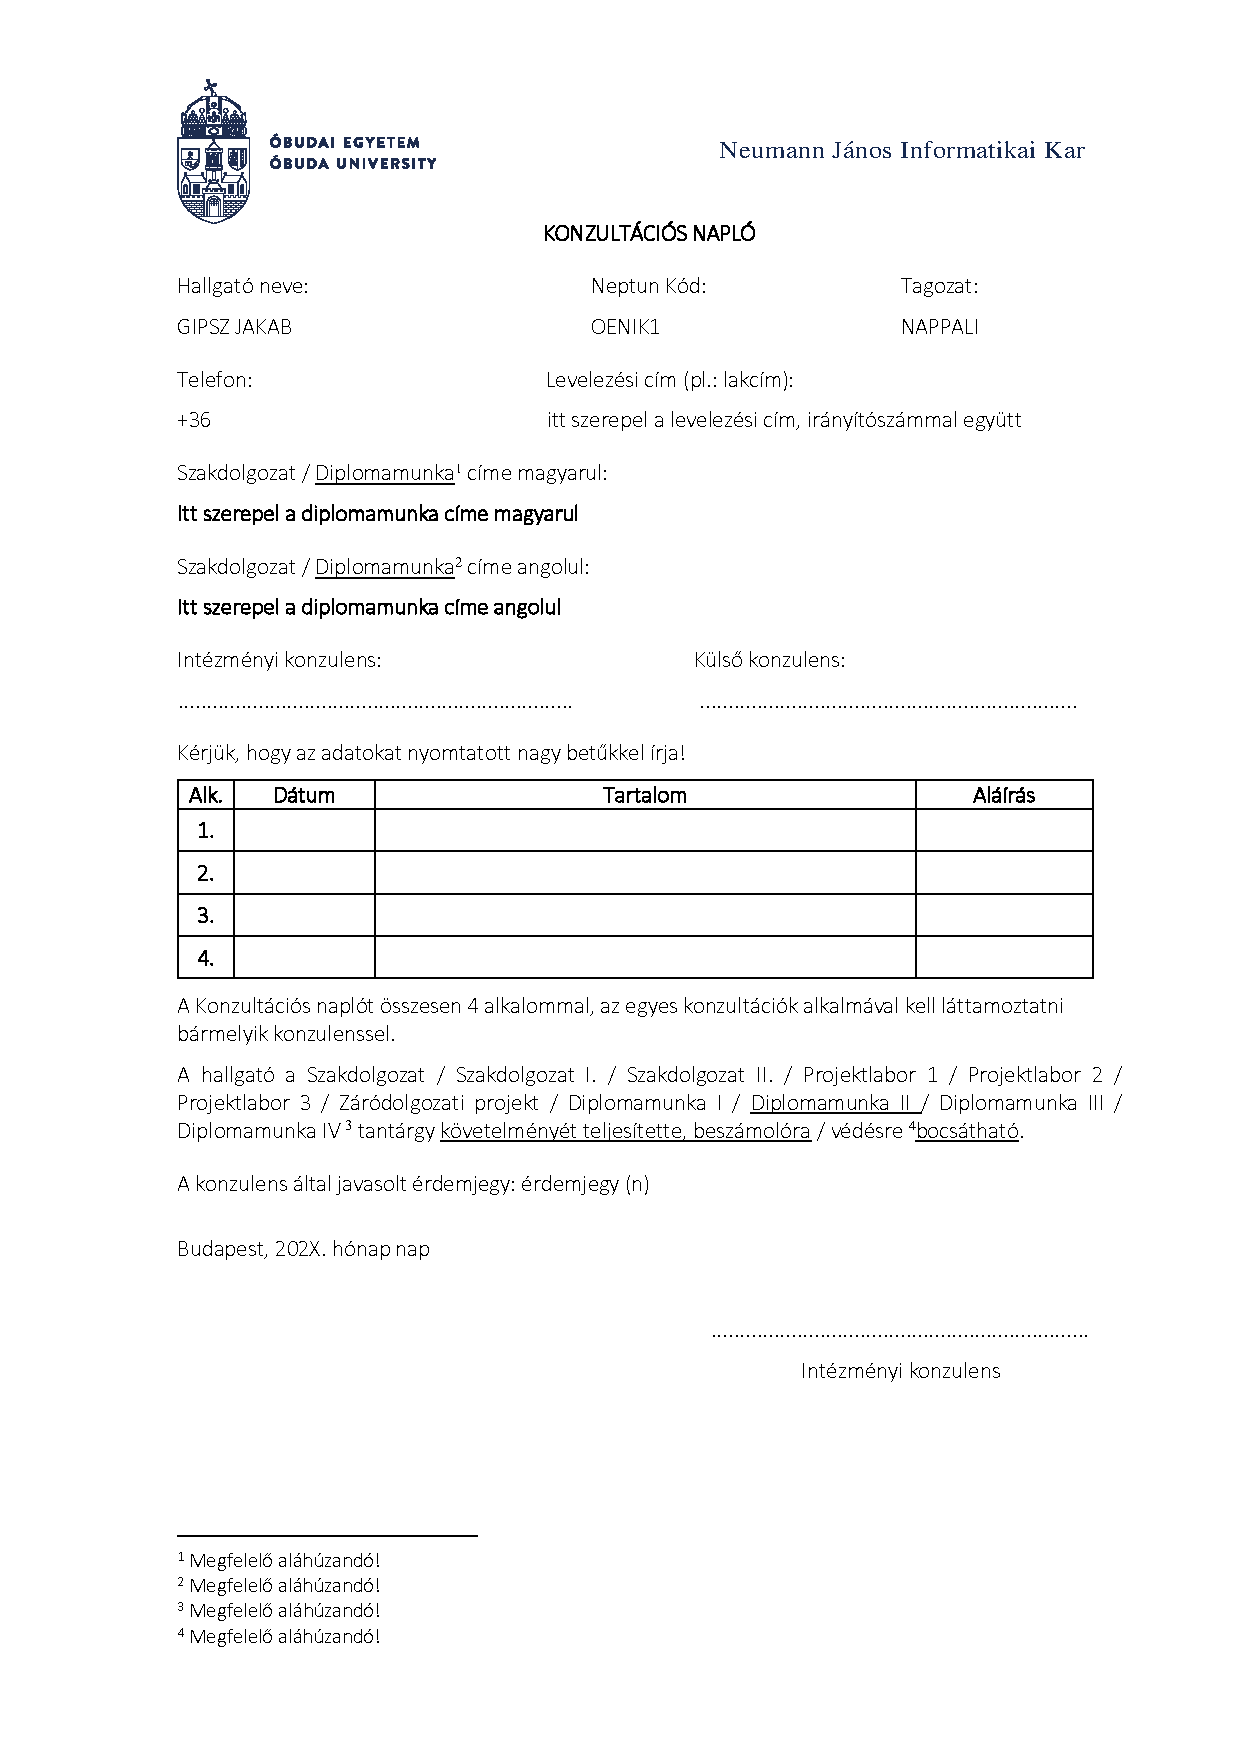
\includepdf[pages=-]{includes/KONZULTACIOS-NAPLO_DM2_NAPPALI 1.pdf}
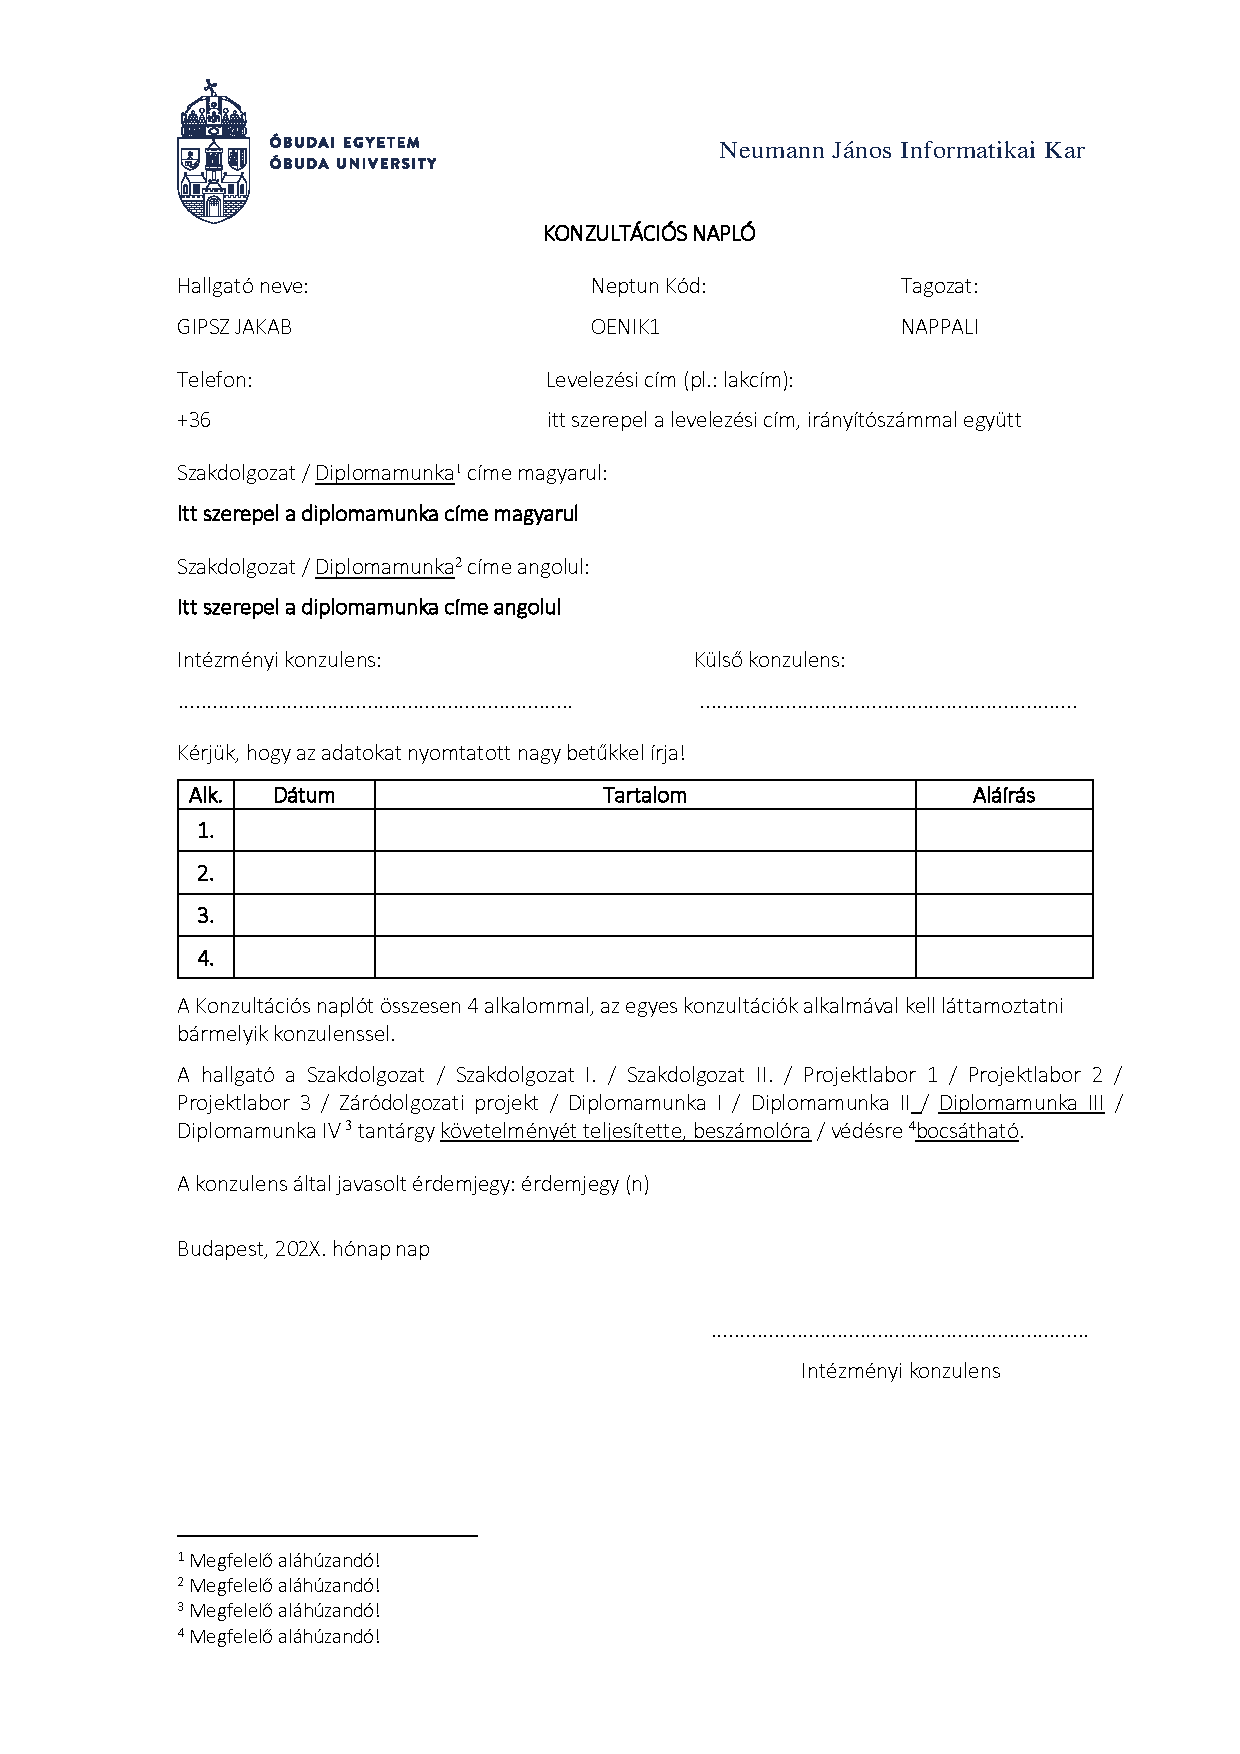
\includepdf[pages=-]{includes/KONZULTACIOS-NAPLO_DM3_NAPPALI 1.pdf}



\section*{ABSZTRAKT}
% Absztrakt magyarul – a szerző írja.

\newpage
\section*{ABSTRACT}
% Abstract in English – a szerző írja.



% TARTALOMJEGYZÉK
\newpage
\pagenumbering{arabic}
\tableofcontents
\newpage


% -----------------------------------------------------

% ITT KELL HOZZÁADNI A FEJEZETEKET, CÍM NAGYBETŰVEL:

\clearpage
\section{BEVEZETÉS}
% 1. fejezet: Bevezetés – a szerző írja.


% A további fejezeteket a szerző veszi fel (a kari útmutató 3. melléklete szerinti felépítésben).










% ------------------------------------------------------

% ÖSSZEFOGLALÓK (útmutató, 3. melléklet 11–12. pont; a magyar 1500–2500 karakter)
\clearpage
\section{ÖSSZEFOGLALÁS}
% Összefoglalás magyarul (1500–2500 karakter) – a szerző írja.


\clearpage
\section{SUMMARY}
% Summary in English – a szerző írja.


% ------------------------------------------------------

% JEGYZÉKEK, INNEN KI LEHET KOMMENTEZNI AMELYIK ESETLEG NEM KELL (de ha van ábra/táblázat akkor kötelező, irodalomjegyzék kötelező, rövidítések opcionális)

\clearpage
\section{IRODALOMJEGYZÉK}
\printbibliography[heading=none]

\clearpage
\renewcommand{\listfigurename}{ÁBRAJEGYZÉK}
\listoffigures

\clearpage
\renewcommand{\listtablename}{TÁBLAJEGYZÉK}
\listoftables

% A rövidítések jegyzéke: az első rövidítés felvétele után a kommentjel törlendő.
% \clearpage
% \section{RÖVIDÍTÉSEK}
% % Rövidítések (acro csomag). Minden rövidítés egy bejegyzés, például:
%
% \DeclareAcronym{SOC}{
%   short = SOC,
%   long  = Security Operations Center
% }
%
% A szövegben: \ac{SOC} (első előfordulásnál teljes név, utána rövidítés), \ac{SOC}-ban (toldalék),
% \acs{SOC} (mindig rövid), \acl{SOC} (mindig teljes). Az első előfordulás legyen toldalék nélkül.
%
% IDE LEHET HOZZÁADNI A RÖVIDÍTÉSEKET:



% MELLÉKLETEK (útmutató, 3. melléklet 14. pont): ha lesz melléklet, a kommentjel törlendő.
% \clearpage
% \section{MELLÉKLETEK}
% % Mellékletek – a szerző állítja össze.






\end{document}